% I²C : Inter-integrated circuit (serial bus)
% VL53L1X : 16x16 Single Photon Avalanche Diode
%           Integrated lens

%%%%%%%%%%%%%%%%%%%%%%%%%%%%%%%%%%%%%%%%%%%%%%%%%%%%%%%%%%%%%%%%%%%%%%%%%%%%%%%

% Informations
\documentclass[a4paper, 11pt]{article}
\title{Un détecteur d'obstacles pour malvoyants}
\author{Arthur Jacquin\\Candidat 27397}
\date{}

% Langue française
\usepackage[utf8]{inputenc}
\usepackage[T1]{fontenc}
\usepackage[frenchb]{babel}

% Couleurs
\usepackage{xcolor}
\definecolor{beaverred}{RGB}{204,0,0}
\definecolor{beaverblue}{RGB}{0,68,204}
\definecolor{beavergreen}{RGB}{0,153,0}

% Figures
\usepackage{caption}
\DeclareCaptionFont{captioncolor}{\color{beaverred}}
\captionsetup{labelfont={captioncolor}}
\DeclareCaptionLabelSeparator{sep}{ : }
\captionsetup{labelsep=sep}
\usepackage{subfig}
\usepackage{tikz}
\usepackage{circuitikz}
\usepackage{pgfplots}
\pgfkeys{/pgf/number format/.cd,1000 sep={\,}}
\pgfplotsset{width=8cm,compat=1.9}
\usepackage{amsmath}

% Code
\usepackage{listings}
\lstdefinestyle{simple}{
    extendedchars=true,
    basicstyle=\ttfamily,
    backgroundcolor=,
    commentstyle=\color{beavergreen},
    keywordstyle=\color{beaverblue},
    numberstyle=\ttfamily\color[rgb]{0.5,0.5,0.5},
    breakatwhitespace=false,
    breaklines=true,
    captionpos=b,
    keepspaces=true,
    numbers=left,
    numbersep=7pt,
    showspaces=false,
    showstringspaces=false,
    showtabs=false,
    tabsize=4,
    columns=fixed
}
\lstset{style=simple}

% Style
\usepackage{hyperref} 
\usepackage{parskip}
\usepackage[toc]{appendix}
\pagestyle{plain}
\usepackage{geometry}
\geometry{includehead, includefoot}
\geometry{top=1.5cm, bottom=1.5cm, left=3cm, right=3cm}
\usepackage[backend=biber]{biblatex}
\addbibresource{biblio.bib}
\usepackage{float}



%%%%%%%%%%%%%%%%%%%%%%%%%%%%%%%%%%%%%%%%%%%%%%%%%%%%%%%%%%%%%%%%%%%%%%%%%%%%%%%

\begin{document}
\maketitle
\tableofcontents
\newpage
\listoffigures
\listoftables
\printbibliography



%%%%%%%%%%%%%%%%%%%%%%%%%%%%%%%%%%%%%%%%%%%%%%%%%%%%%%%%%%%%%%%%%%%%%%%%%%%%%%%

\newpage \section{Introduction}

\subsection{Contexte}

\par Avec plusieurs dizaines de millions de personnes touchées selon l'Organisation Mondiale de la Santé \cite{oms}, et potentiellement trois fois plus d'ici 2050 selon le journal médical The Lancet \cite{thelancet}, la cécité est une problématique majeure de santé publique. Les conséquences des déficiences visuelles sont lourdes et nombreuses, par exemple dans la mobilité.

Les solutions les plus communes, comme la canne blanche ou les chiens-guides, présentent toutes des problèmes : la canne a une portée limitée, le chien-guide nécessite une logistique plus importante. De plus, ces solutions ne permettent pas de détecter certains obstacles, notamment ceux situés en hauteur (au dessus du bassin).

Pour répondre à ces problématiques, des entreprises commercialisent des cannes électroniques permettant aux déficients visuels de détecter les obstacles les plus proches. On peut citer CECIAA, Visioptronic ou GoSense, avec respectivement l'Ultracane \cite{ultracane}, Tom Pouce \cite{tompouce} et Rango. La perception de l'environnement proche est effectuée par des capteurs de distance, dont la portée dépasse dix mètres pour Tom Pouce. Les informations sont ensuite communiquées à l'utilisateur par le biais de vibrations. Cependant, ces solutions sont très peu démocratisées car très onéreuses (environ 1000 euros pour l'Utracane et 5000 euros pour Tom Pouce) et complexes à prendre en main : pour Tom Pouce, une formation de 30 heures semble nécessaire, pour des résultats partiellement convaincants \cite{formation}. De plus, les cannes sont visuellement discriminantes.

\begin{figure}[H]
\centering
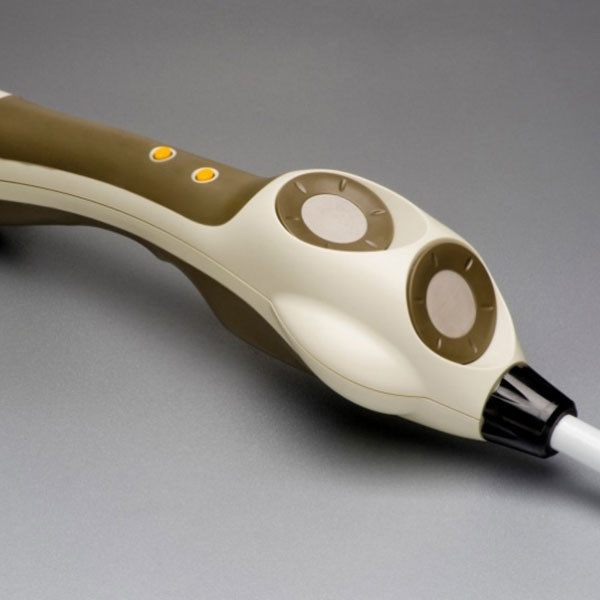
\includegraphics[height=6cm]{images/ultracane.jpg}
\caption{L’UltraCane (CECIAA, 1055 €)}
\end{figure}

De nombreuses recherches s'intéressent aujourd'hui à l'amélioration des capteurs de distance, en raison de la multiplicité de leurs applications, du domaine médical aux voitures autonomes. Concernant les dispositifs pour déficience visuelle, on trouve dans la littérature l'utilisation de différents types de capteurs : capteurs à ultrasons \cite{ultrasons}, caméra pour scanner l'environnement \cite{camera}, capteurs utilisant un radar à ondes millimétriques \cite{radar} ou capteurs LIDAR (LIght Detection And Ranging) \cite{lidar} émettant un faisceau laser. Pour plus de polyvalence, des dispositifs combinant plusieurs technologies de capteurs ont également été étudiés \cite{multicapteur}.


\subsection{Objectif du TIPE}

\par  L’objectif de ce TIPE est de proposer une alternative à ces dispositifs d'aide à la mobilité. L'accent sera mis sur le caractère \textit{open-source} du projet, ainsi que sur son accessibilité économique et technique.

\par Voici le dispositif envisagé : un capteur déterminerait la distance de l'obstacle le plus proche, puis l'information serait communiquée à l'utilisateur par un vibreur. Les vibrations seraient d'autant plus fortes que l'obstacle est proche, et s'arrêteraient pour un obstacle situé à plus de 2 mètres de distance.

\par L'appareil se tiendrait dans une main. Le faisceau de détection serait volontairement très directif : l'idée est de balayer l'environnement avec des petits mouvements de main (mode par balayages). Cela laisse à l'utilisateur le contrôle sur les zones à sonder, et permet de détecter les obstacles en hauteur.


\subsection{Cahier des charges fonctionnel}

\par L'établissement du cahier des charges fonctionnel reste la première étape de ce projet, puisqu'il permet de guider la conception du dispositif.

\par Certaines critères identifiés relèvent du bon fonctionnement de l'appareil. Cela comprend la détection de l'obstacle le plus proche et la communication avec l'utilisateur.

\par Pour le mode envisagé d'utilisation par balayages, la détection des obstacles se doit d'être rapide et directive. Concernant l'interface utilisateur, il semble primordial de mettre en valeur la distance de l'obstacle le plus proche par la variation, c'est-à-dire le caractères \textit{progressif} de l'interface.

\par Les autres critères identifiés lient le dispositif technique et son environnement d'utilisation. Étant destiné à un usage commun et quotidien, l'appareil créé doit être robuste, et simple d'utilisation, donc compact et maniable. Par ailleurs, pour que chacun puisse reproduire le dispositif, il importe qu'il soit abordable financièrement et que sa fabrication ne demande pas de compétences techniques préalables.

\bigskip

\begin{table}[h!]
\centering
\begin{tabular}{llc}
\hline
{\bf Fonction} & {\bf Critère} & {\bf Valeur} \\
\hline
Détecter la distance de & Portée & \textgreater 3 m \\
l'obstacle le plus proche & Faisceau de détection & \\
 & Réactivité & \textgreater 5 Hz \\
\hline
Traiter l'information & Cohérence & \\
\hline
Communiquer l'information & Clarté & \\
à l'utilisateur & Progressivité & \\
\hline
Être reproductible & Accessibilité économique & \textless 50 € \\
 & Accessibilité technique & \\
\hline
Être ergonomique & Compacité & \\
 & Maniabilité & \\
 & Robustesse & \\
\hline
\end{tabular}
\caption{Cahier des charges fonctionnel}
\end{table}



%%%%%%%%%%%%%%%%%%%%%%%%%%%%%%%%%%%%%%%%%%%%%%%%%%%%%%%%%%%%%%%%%%%%%%%%%%%%%%%

\newpage \section{Choix du capteur de distance}

\par Le capteur de distance est l'un des éléments centraux du dispositif. Il a une grande importance dans la qualité du produit final. Son choix est donc primordial : nous allons donc en tester plusieurs.

\par Le fonctionnement des modèles testés est identique, et repose sur le principe d'écholocalisation. Une onde, dont la nature dépend du capteur, est ponctuellement émise par le capteur, se réfléchit sur les obstacles, puis est reçue par le capteur. On remarque que la distance parcourue par l'onde entre son émission et sa réception est égale au double de la distance du capteur à l'ostacle. On peut ainsi on déduire la distance $d$ de l'obstacle, en notant $v$ la vitesse de l'onde dans le milieu et $\Delta t$ le temps séparant la réception de l'émission de l'onde :

\begin{equation}
d = \frac{v \cdot \Delta t}{2}
\end{equation}

\subsection{Modèles testés}

\par Comme le montre les recherches bibliographiques préalables, 3 types de capteurs sont régulièrement utilisés dans la détection d'obstacles : capteurs ultrasons, infrarouges, ou laser.

\par Les capteurs infrarouges ont immédiatement été écartés du projet, jugés trop onéreux. Les modèles suivants ont été choisis pour représenter les différentes natures d'ondes possibles. Pour une nature d'onde donnée, la portée annoncée par les constructeurs des capteurs a permis de faire la présélection suivante :

\begin{table}[h!]
\centering
\begin{tabular}{r|ccc}
{\bf Capteur} & VL53L1X & \multicolumn{2}{c}{MB1013} \\
 & 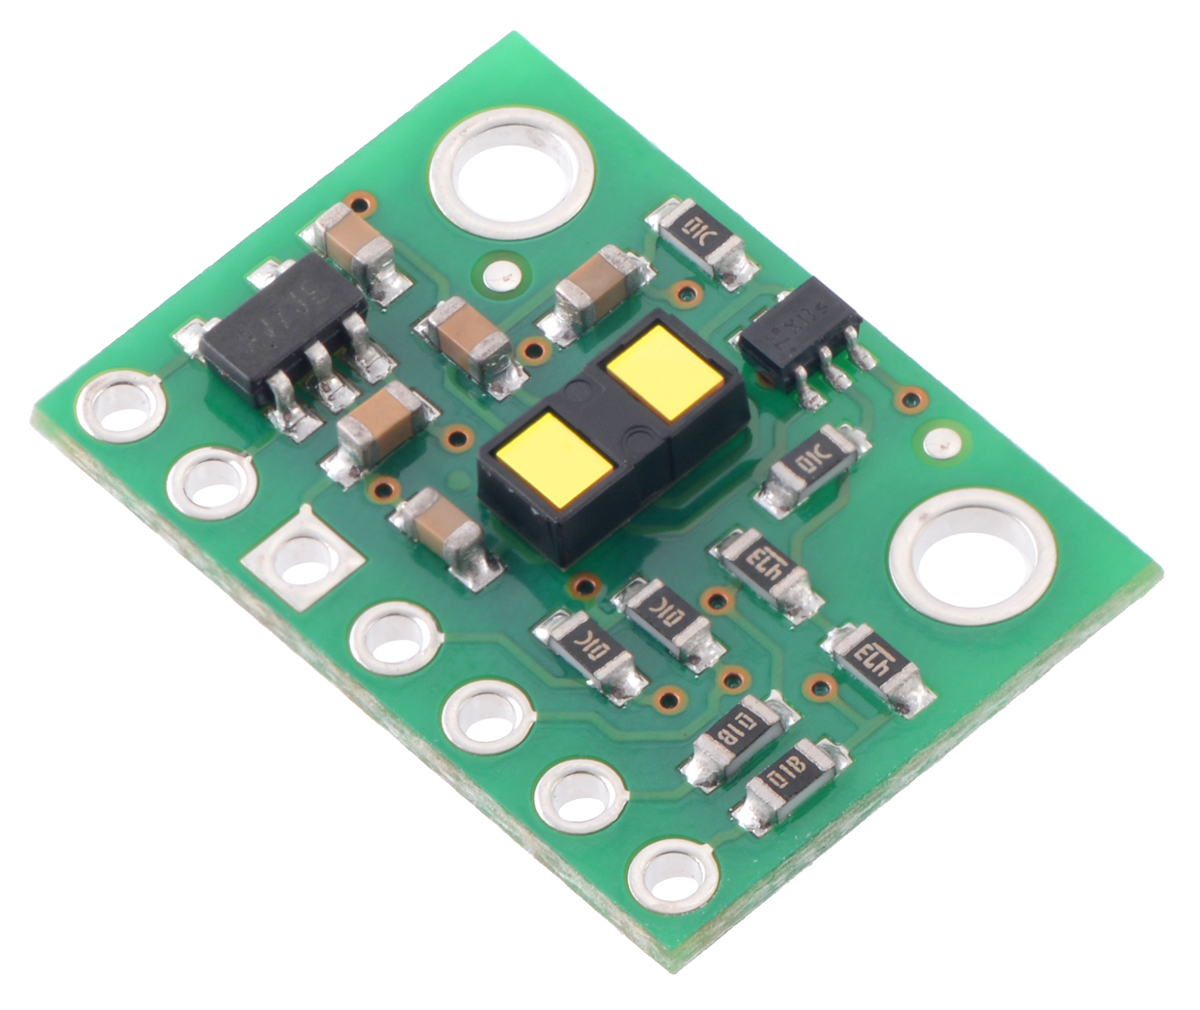
\includegraphics[height=2.5cm]{images/VL53L1X.jpg} & \multicolumn{2}{c}{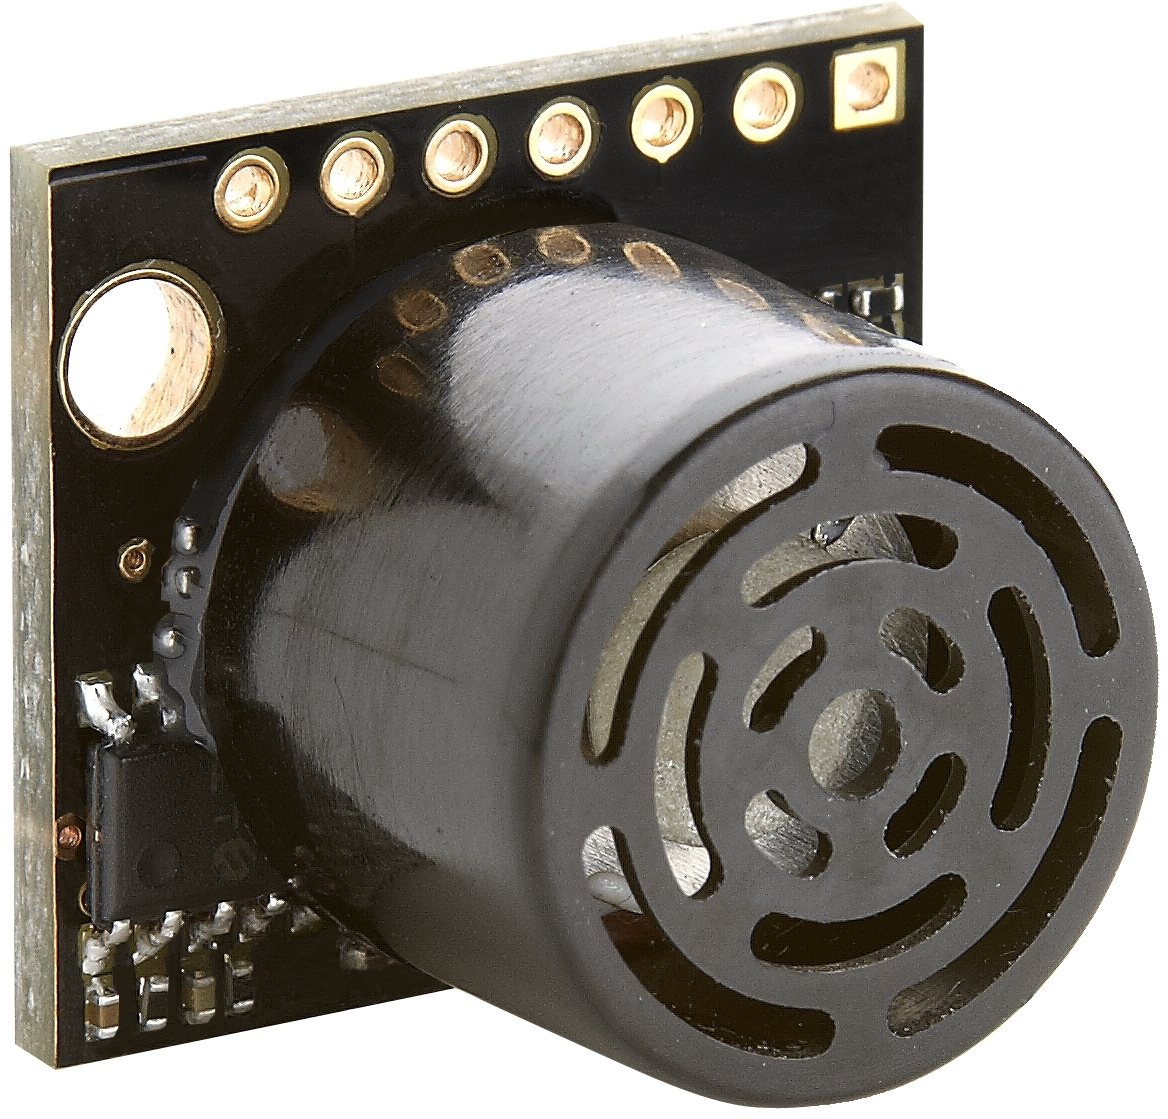
\includegraphics[height=2.5cm]{images/maxsonar_ez1_mb1013.jpg}} \\
{\bf Type d'onde} & Lumineuse & \multicolumn{2}{c}{Sonore} \\
{\bf Domaine} & Infrarouge (940 nm) & \multicolumn{2}{c}{Ultrasonore (42 kHz)} \\
{\bf Prix} & 19,40 € & \multicolumn{2}{c}{39,90 €} \\
{\bf Interface} & I²C & Analogique & MLA \\
 &
    \begin{tikzpicture}
    \footnotesize
    \draw (0, 0) rectangle (1.3, 1.8);
    \foreach \y in {0.13,0.384,...,1.8} \draw (0.13, \y) circle (0.085);
    \draw (0.045, 1.061) rectangle (0.215, 1.231);
    \draw[color=blue, thick] (0.13, 1.4) -- +(0.3,0) node[anchor=west] {5V};
    \draw[color=black, thick] (0.13, 1.146) -- +(0.3,0) node[anchor=west] {GND};
    \draw[color=beaverred, thick] (0.13, 0.892) -- +(0.3,0) node[anchor=west] {SDA};
    \draw[color=beaverred, thick] (0.13, 0.638) -- +(0.3,0) node[anchor=west] {SCL};
    \end{tikzpicture}
    &
    \begin{tikzpicture}
    \footnotesize
    \draw (0, 0) rectangle (2, 2.2);
    \foreach \y in {0.13,0.384,...,1.8} \draw (0.13, \y) circle (0.085);
    \draw (0.045, 0.045) rectangle (0.215, 0.215);
    \draw[color=black, thick] (0.13, 1.654) -- +(0.3,0) node[anchor=west] {GND};
    \draw[color=blue, thick] (0.13, 1.4) -- +(0.3,0) node[anchor=west] {5V};
    \draw[color=beaverred, thick] (0.13, 0.638) -- +(0.3,0) node[anchor=west] {A0};
    \end{tikzpicture}
    & 
    \begin{tikzpicture}
    \footnotesize
    \draw (0, 0) rectangle (2, 2.2);
    \foreach \y in {0.13,0.384,...,1.8} \draw (0.13, \y) circle (0.085);
    \draw (0.045, 0.045) rectangle (0.215, 0.215);
    \draw[color=black, thick] (0.13, 1.654) -- +(0.3,0) node[anchor=west] {GND};
    \draw[color=blue, thick] (0.13, 1.4) -- +(0.3,0) node[anchor=west] {5V};
    \draw[color=beaverred, thick] (0.13, 0.384) -- +(0.3,0) node[anchor=west] {D3};
    \end{tikzpicture} \\
\end{tabular}
\caption{Modèles de capteurs de distance testés}
\end{table}

\par Le VL53L1X utilise donc un laser (de classe 1, donc inoffensif) de longueur d'onde invisible à l'homme. Il peut communiquer avec le microcontrôleur \textit{via} l'interface I²C, utilisant les broches \texttt{SDA} et \texttt{SDL} du microcontrôleur. Dévellopé par ST Microelectronics, on utilise ici une version soudée sur une carte, pour faciliter la connection à un microcontrôleur. 

\par Le capteur MB1013, de la gamme HRLV-MaxSonar-EZ1 dévellopée par Maxbotic, utilise les ondes ultrasonores. Il est déjà fixé à une plaque. Il peut communiquer de deux façons : analogique, en le connectant à une broche analogique du microcontrôleur, et en modulation de largeur d'amplitude (MLA), processus détaillé dans la partie correspondante, en le connectant à une broche digitale du microcontrôleur. Ces deux modes de communication seront testés.


\subsection{Détermination du faisceau de détection}

\par La première étape des tests consiste à déterminer le faisceau de détections des capteurs, c'est-à-dire la zone dans laquelle un obstacle est détecté (quelque soit la précision de la mesure de distance).

\begin{figure}[H]
\centering
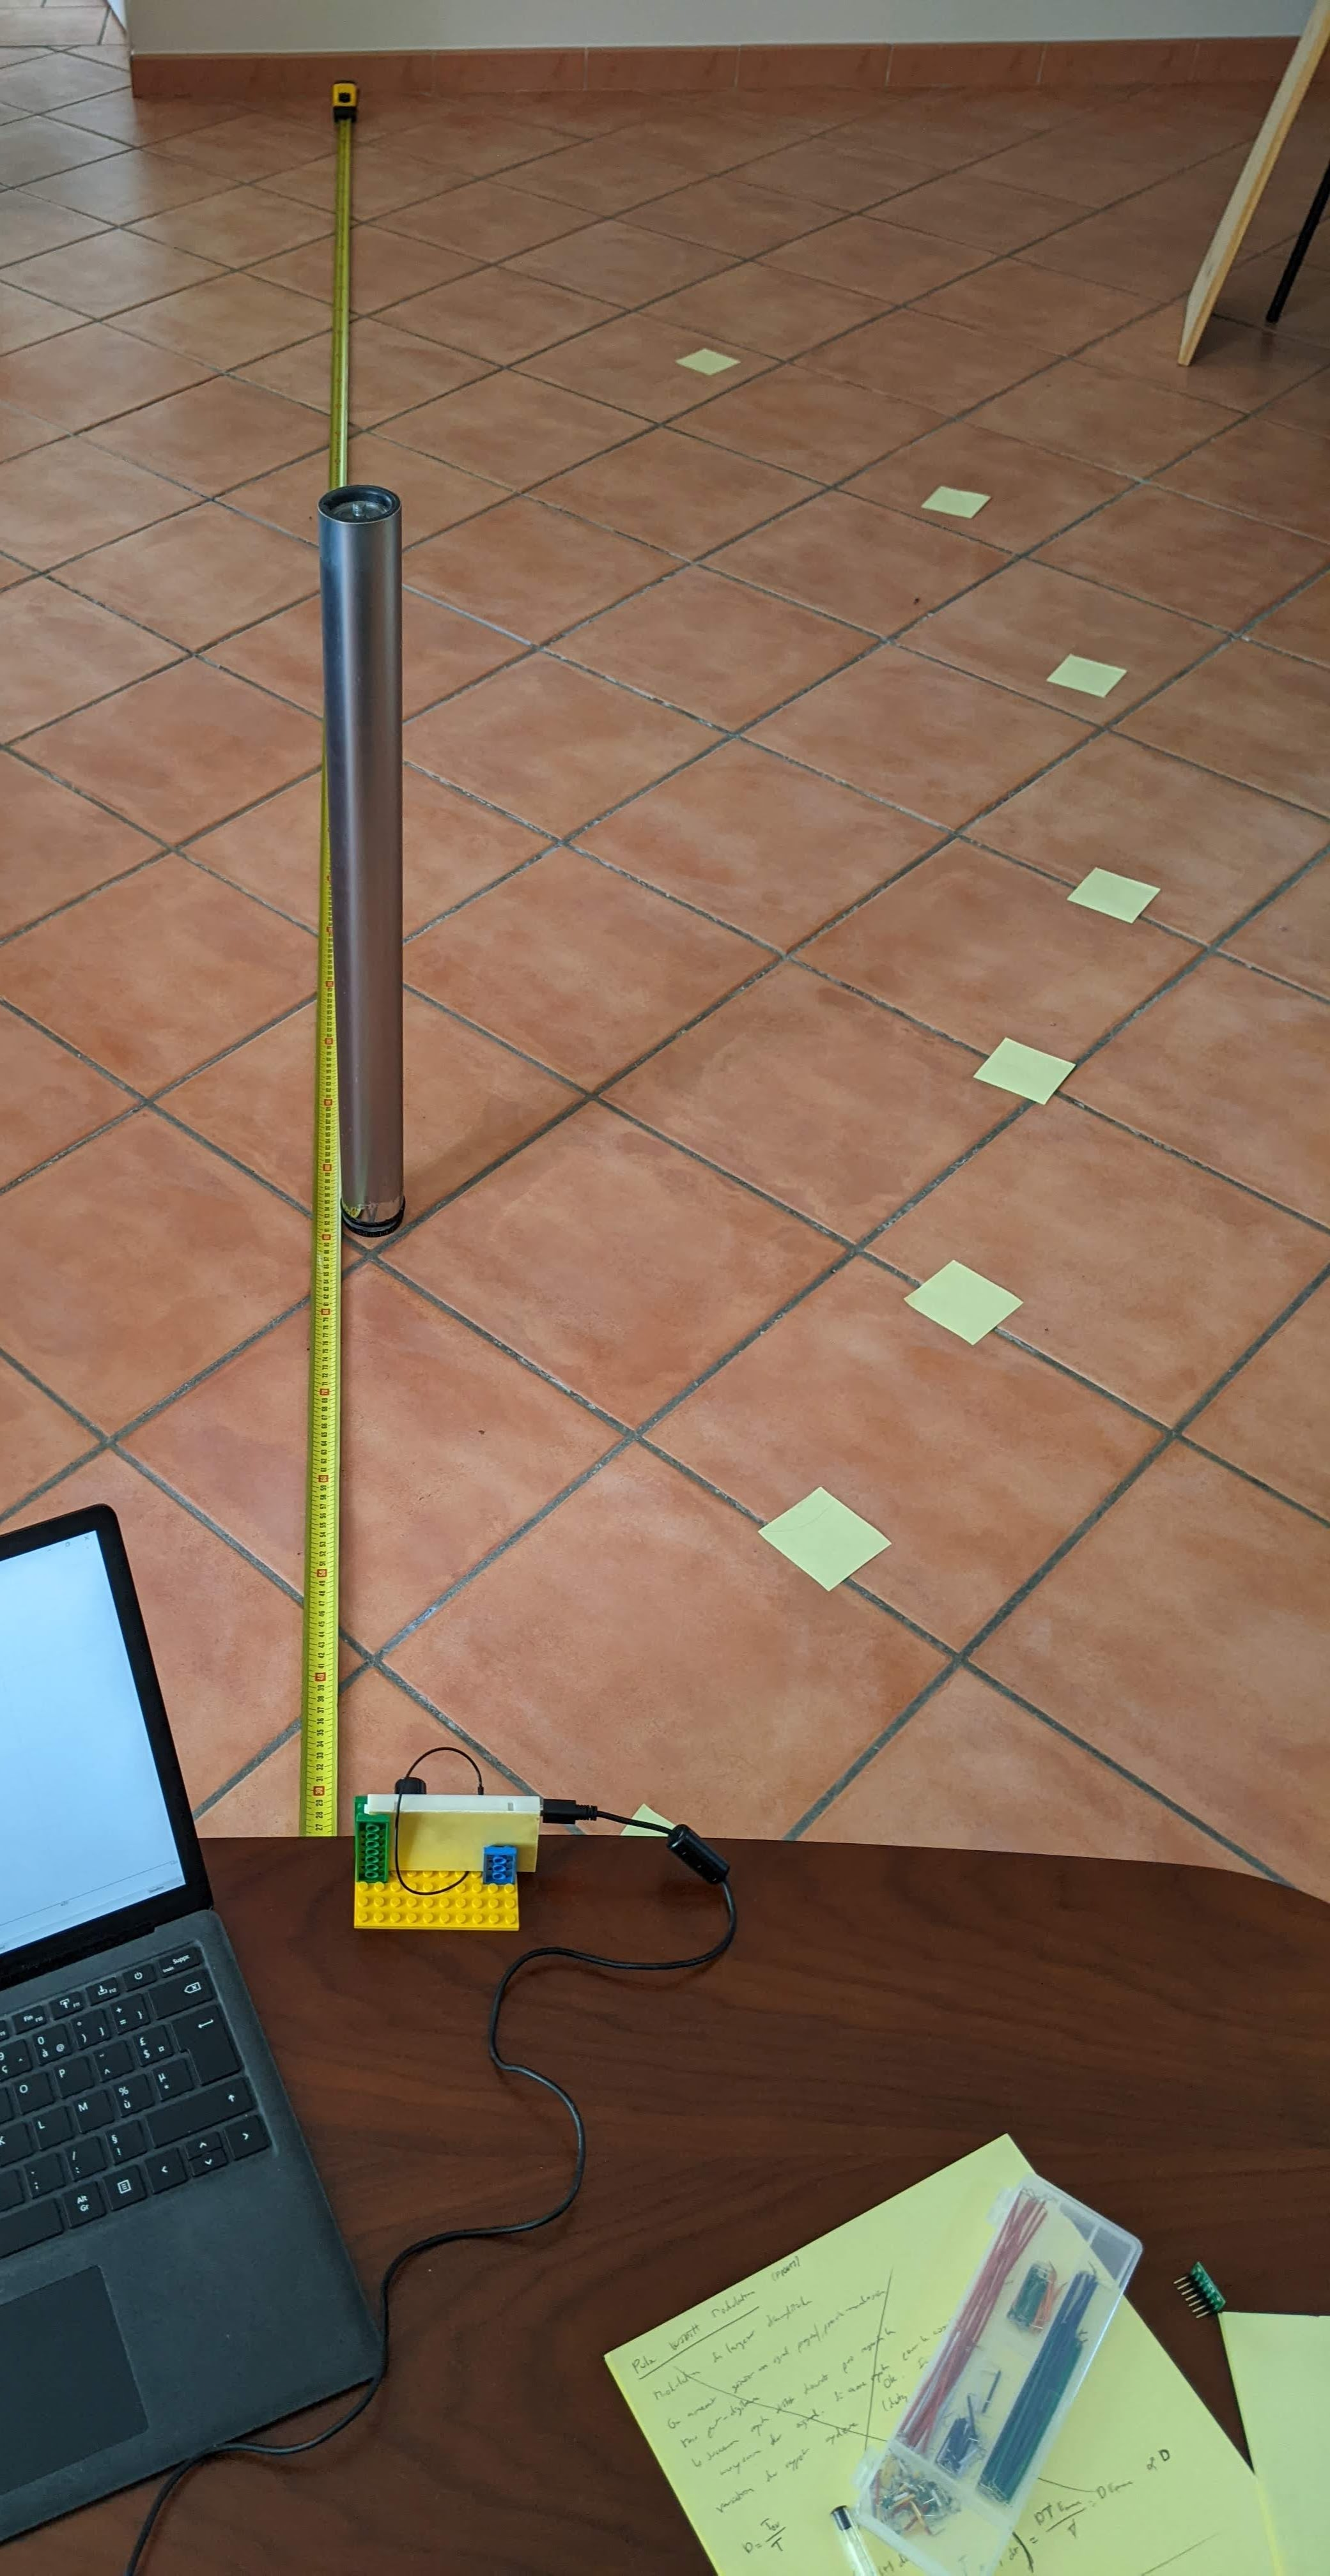
\includegraphics[height=10cm]{images/faisceau.jpg}
\caption{Dispositif de test}
\end{figure}

\par Les mesures se font dans un environnement dégagé. Pour plusieurs distances $d_{axiale}$, on place un obstacle cylindrique, de diamètre 6 cm, dans l'axe de détection du capteur testé, puis on le déplace perpendiculairement à cet axe, et on note la distance $d_{radiale}$ à l'axe pour laquelle le capteur ne détecte plus l'obstacle. Le choix du diamètre de l'obstacle est censé refléter la taille minimale des obstacles communs dans l'espace public, par exemple des poteaux.

\par L'émission des ondes étant invariante par rotation autour de l'axe de détection, la zone de détection conserve cette invariance. Pour une distance $d_{axiale}$ donnée, une seule mesure de $d_{radiale}$ suffit pour caractériser le faisceau.

\begin{figure}[H]
\centering
\begin{tikzpicture}
\begin{axis}[
    legend cell align = {left},
    legend pos=north west,
    width=\textwidth,
    height=10cm,
    xmin=0, xmax=3.5,
    ymin=-1.2, ymax=1.5,
    xtick distance=1,
    ytick distance=1,
    grid=both,
    grid style=dashed,
    xlabel={$d_{axiale}$ (m)},
    ylabel={$d_{radiale}$ (m)},
]
\addplot[line width=1pt, color=beaverred, mark=x] coordinates {
    (2.5,-0.13)(2,-0.14)(1.5,-0.13)(1.2,-0.15)(0.9,-0.16)(0.6,-0.10)
    (0.3,-0.03)(0.3,0.03)(0.6,0.10)(0.9,0.16)(1.2,0.15)(1.5,0.13)(2,0.14)(2.5,0.13)};
\addplot[line width=1pt, color=beaverblue, mark=x] coordinates {
    (0.3,0.25)(0.6,0.43)(0.9,0.59)(1.2,0.72)(1.5,0.88)(2,0.97)
    (2.5,0.86)(3,0.72)(3.2,0)(3,-0.72)(2.5,-0.86)(2,-0.97)(1.5,-0.88)
    (1.2,-0.72)(0.9,-0.59)(0.6,-0.43)(0.3,-0.25)};
\addplot[line width=1pt, color=beavergreen, mark=x] coordinates {
    (0.3,0.22)(0.6,0.40)(0.9,0.57)(1.2,0.69)(1.5,0.86)(2,0.95)(2.5,0.88)
    (3,0.59)(3.3,0)(3,-0.59)(2.5,-0.88)(2,-0.95)(1.5,-0.86)
    (1.2,-0.69)(0.9,-0.57)(0.6,-0.40)(0.3,-0.22)};
\legend{
    VL53L1X,
    MB1013 - Analogique,
    MB1013 - MLA}
\draw[line width=1pt,->] (axis cs:0,0) -- (axis cs:0.2,0);
\end{axis}
\end{tikzpicture}
\caption{Zone détectée par le capteur placé à l'origine}
\label{faisceau}
\end{figure}

\par Les résultats, en figure \ref{faisceau}, sont cohérents avec la nature des ondes utilisées : le laser est plus directif que les ondes sonores, bien que le VL53L1X intègre des lentilles (une pour l'émission, une autre pour la réception) permettant d'étendre le champ de vision à 27°.

\par L'incertitude des mesures est évaluée à 2 cm pour $d_{axiale}$, et à 5 cm pour $d_{radiale}$. Le mode de communication du MB1013 n'a que peu d'influence. La portée du VL53L1X semble plus limitée que celle du MB1013, sur ce test, mais cela est dû au faible diamètre de l'obstacle. En effet, le VL53L1X reste précis (à 5 cm près) jusqu'à plus de 4 mètres lorsqu'il fait face à un mur.


\subsection{Précision des capteurs}

\par Le deuxième test mesure la précision des capteurs. On déplace un coussin (mou, analogue au vêtements d'un piéton) carré de 35 cm de coté le long de l'axe de détection, et on relève la distance de détection du capteur pour la comparer à la distance réelle de l'obstacle.

\begin{figure}[H]
\centering
\begin{tikzpicture}
\begin{axis}[
    width=\textwidth,
    height=10cm,
    xlabel={Distance réelle (mm)},
    ylabel={Distance mesurée (mm)},
    xmin=0, xmax=4200,
    ymin=0, ymax=4200,
    xtick={0,1000,2000,3000,4000},
    ytick={0,1000,2000,3000,4000},
    legend cell align = {left},
    legend pos=south east,
    ymajorgrids=true,
    grid style=dashed,
]
\addplot[color=beaverred, line width=1pt, mark=x]
    coordinates {(600,602)(900,895)(1200,1186)(1500,1499)
        (2000,2030)(2500,2600)(3000,3200)(3500,3700)};
\addplot[color=beaverblue, line width=1pt, mark=x]
    coordinates {(600,595)(900,890)(1200,1195)(1500,1495)
        (2000,1980)(2500,2470)(3000,2970)(3500,3450)(4000,3915)};
\addplot[color=beavergreen, line width=1pt, mark=x]
    coordinates {(600,597)(900,883)(1200,1198)(1500,1482)
        (2000,1980)(2500,2466)(3000,2945)(3500,3450)(4000,3950)};
\addplot[dashed] coordinates {(0,0)(4200,4200)};
\legend{
    VL53L1X,
    MB1013 - Analogique,
    MB1013 - MLA}
\end{axis}
\end{tikzpicture}
\caption{Mesures de distance}
\end{figure}

\par Le MB1013 semble plus précis. La précision du capteur n'est cependant pas un facteur de choix déterminant pour ce projet : les écarts peuvent être corrigés algorithmiquement. L'important est que la distance mesurée augmente bien progressivement avec la distance de l'obstacle.


\subsection{Réactivité des capteurs}

\par La réactivité a été identifié comme facteur clé. Pour la tester, on place un obstacle à environ 1 mètre du capteur, et on laisse tomber, à $t_0$, une feuille A4 30 cm en devant du capteur. On s'attend à ce que la mesure de distance du capteur passe brutalement de 100 cm (obstacle en arrière plan) à 30 cm (feuille en train de tomber), puis de nouveau à 100 cm (chute de la feuille terminée).

\begin{figure}[H]
\centering
\begin{tikzpicture}
\begin{axis}[
    width=\textwidth,
    height=10cm,
    xlabel={Temps (s)},
    ylabel={Distance de l'obstacle (mm)},
    xmin=0, xmax=1.3,
    ymin=0, ymax=1200,
    xtick={0, 0.3, 1},
    xticklabels = {0, $t_0$, 1},
    ytick={0, 300, 600, 900, 1200},
    legend cell align = {left},
    legend pos=south east,
    ymajorgrids=true,
    grid style=dashed,
]
\addplot[color=beaverred, line width=1pt, mark=x]
    coordinates {(0.05,990)(0.1,982)(0.15,989)(0.2,998)
        (0.25,993)(0.3,996)(0.35,589)(0.4,295)(0.45,309)
        (0.5,1021)(0.6,987)(0.65,990)(0.7,994)};
\addplot[color=beaverblue, line width=1pt, mark=x]
    coordinates {(0,970)(0.1,970)(0.2,970)(0.3,970)
        (0.4,855)(0.5,825)(0.6,830)(0.7,825)(0.8,835)
        (0.9,850)(1,980)(1.1,970)(1.2,975)};
\addplot[color=beavergreen, line width=1pt, mark=x]
    coordinates {(0,983)(0.1,977)(0.2,978)(0.3,977)
        (0.4,818)(0.5,818)(0.6,976)(0.7,977)(0.8,977)};
\addplot[dashed] coordinates {(0,1000)(1.3,1000)};
\node at (axis cs:1.3,1000) [anchor=south east] {Obstacle en arrière plan};
\addplot[dashed] coordinates {(0.3,0)(0.3,1200)};
\legend{
    VL53L1X,
    MB1013 - Analogique,
    MB1013 - MLA}
\end{axis}
\end{tikzpicture}
\caption{Détection d'une feuille A4 lachée à 30 cm du capteur à $t_0$}
\end{figure}

\par Les résultats du VL53L1X sont très convaincants. En revanche, les mesures du MB1013 semblent erratiques.


\subsection{Conclusion}

\par Dans tous les tests réalisés, le mode de communication du MB1013 a semblé peu significatif. On se contente donc de comparer les deux capteurs indépendamment du mode de communication :

\begin{table}[h!]
\centering
\begin{tabular}{r|cc}
{\bf Capteur} & VL53L1X & MB1013 \\
{\bf Portée} & ++ & +++ \\ 
{\bf Faisceau} & Directif & Large \\
{\bf Précision} & Suffisante & Suffisante \\
{\bf Réactivité} & +++ & + \\
{\bf Prix} & 19,40 € & 39,90 € \\
\end{tabular}
\caption{Récapitulatif des tests}
\end{table}

\par Malgré un petit manque de précision face au MB1013, on choisi le VL53L1X. Plus réactif, plus directif, et suffisament précis pour détecter la progressivité dans la distance des obstacles, ce capteur est plus adapté au mode par balayages envisagé pour le dispositif.

\par L'utilisation du VL53L1X a par la suite mené à l'identification d'un léger bruit dans les mesures. Pour l'éliminer, on effectue (algorithmiquement) une moyenne glissante sur 3 points (ce qui correspond à 0,15 s). Un traitement du signal plus poussé a été envisagé (notamment le filtre de Kalman), mais abandonné à cause des limitations techniques et du besoin de réactivité. Par ailleurs, la moyenne glissante suffit à lisser les mesures.



%%%%%%%%%%%%%%%%%%%%%%%%%%%%%%%%%%%%%%%%%%%%%%%%%%%%%%%%%%%%%%%%%%%%%%%%%%%%%%%

\newpage \section{Élaboration de l'interface utilisateur}

\par Une fois l'information (distance de l'obstacle le plus proche) acquise, le dispositif doit la transmettre à l'utilisateur. Un signal sonore a été envisagé, mais s'est vite révélé désagréable à l'utilisation, et peut isoler l'utilisateur de son environnement.

\par Le choix de l'interface s'est naturelement porté sur les vibrations, solution classique parmis les dispositifs personnels de détection d'obstacles. Encore fois, on teste différents vibreurs. 

\begin{table}[h!]
\centering
\begin{tabular}{cccc}
Vibreur Gotronic & VPM2 & Gravity & SMD \\
  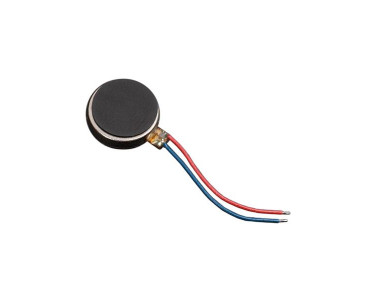
\includegraphics[width=2.3cm]{images/gotronic_vib.jpg}
& 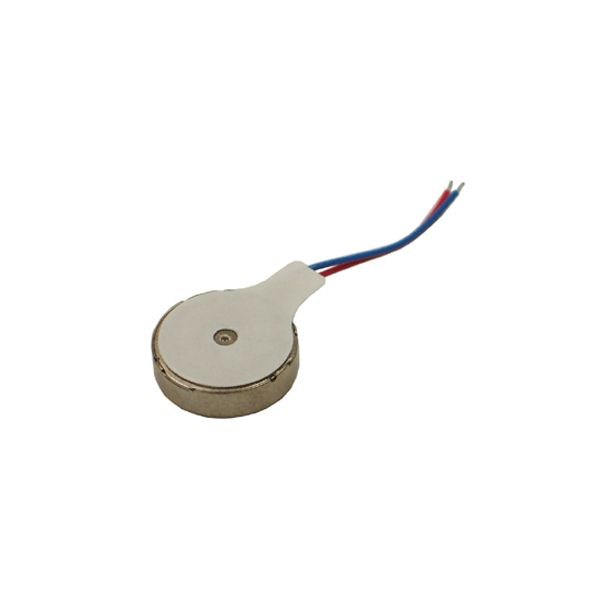
\includegraphics[width=2.3cm]{images/vpm2.jpg}
& 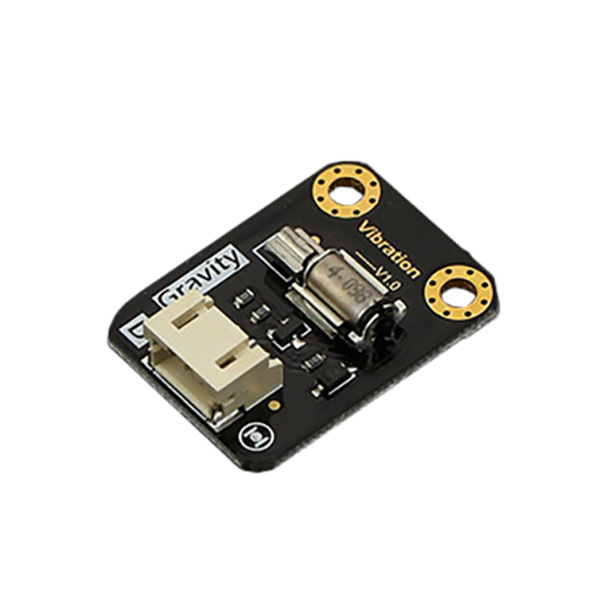
\includegraphics[width=2.3cm]{images/gravity.jpg}
& 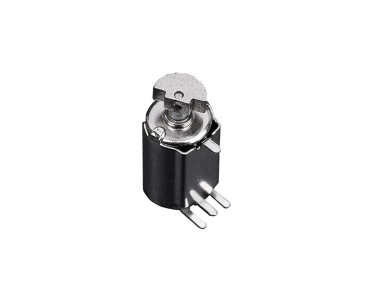
\includegraphics[width=2.3cm]{images/smd.jpg} \\
1,30 € & 4,20 € & 2,60 € & 1,30 € \\
\end{tabular}
\caption{Modèles de vibreurs testés}
\end{table}


\subsection{Modulation de largeur d'amplitude}

\par Les vibreurs sont de simples moteurs, faisant tourner des disques au barycentre désaxé pour générer les vibrations. La première question qui se pose est la façon dont on fait varier l'intensité de la vibration. En effet, on aimerait une amplitude de vibration décroissante avec la distance de l'obstacle, mais le microcontrôleur ne permet que de fixer une tension maximale $E_0$ ou nulle sur ses broches digitales.

\par Pour obtenir, à partir d'un ensemble discret de valeurs, un signal pseudo-analogique, c'est-à-dire à valeurs dans une plage continue de valeurs, on utilise le principe de modulation de largeur d'amplitude (MLA en français, \textit{PWM} pour \textit{Pulse Width Modulation} en anglais).

\par Les vibreurs se comportant comme des filtres passe-bas, on effectue une succession assez rapide de valeurs à ces états discrets, de façon à obtenir une composante continue, c'est à dire la moyenne du signal, à la tension souhaitée. Le microcontrôleur permet de générer de tels signaux à une fréquence de 490 Hz.

\par En pratique, on génère un signal créneau fixé en position "haute" ($E = E_0$) pendant une durée $T_{on}$ de la période $T$, et en position "basse" ($E = 0$) pendant le reste de la période. On note alors $D = \frac{T_{on}}{T}$ le rapport cyclique ({\it duty cycle} en anglais).

\begin{figure}[H]
\centering
\begin{tikzpicture}
\draw[step=1cm,gray,very thin] (0,0) grid (7.5,3.5);
\draw[->, line width=2pt] (0,0) -- (0,3.5) node[anchor=west] {$E(t)$};
\draw (1pt,0) -- (-1pt,0) node[anchor=east] {$0$};
\draw (1pt,3) -- (-1pt,3) node[anchor=east] {$E_0$};
\draw[->, line width=2pt] (0,0) -- (7.5,0) node[anchor=north west] {$t$};
\draw (0,1pt) -- (0,-1pt) node[anchor=north] {$0$};
\draw (2,1pt) -- (2,-1pt) node[anchor=north] {$T_{on}$};
\draw (5,1pt) -- (5,-1pt) node[anchor=north] {$T$};
\draw[color=beaverred, line width=2pt] (0,0) -- (0,3) -- (2,3) -- (2,0)
    -- (5,0) -- (5,3) -- (7,3) -- (7,0) -- (7.3,0);
\end{tikzpicture}
\caption{Modélisation du signal créneau (pour un rapport cylique de 0.4)}
\end{figure}

\par Après calcul, la composante continue du signal (correspondant à la moyenne temporelle dans la décomposition de Fourier) est proportionnelle au rapport cyclique. La génération du signal décrit est une fonctionnalité integrée au microcontrôleur : il suffit de préciser le rapport $D$ pour appliquer la tension choisie au vibreur. C'est aussi avec cette méthode que le capteur MB1013 communique la distance mesurée de l'obstacle le plus proche dans le mode de communication MLA.

\begin{equation}
<E(t)> \;
    = \frac{1}{T} \int_0^T{E(t) \: dt}
    = \frac{1}{T} \left(\int_0^{T_{on}}{E_0 \: dt} + \int_{T_{on}}^T{0 \: dt} \right)
    = D \cdot E_0
\end{equation}


\subsection{Courbes intensité-ressenti}

\par Le ressenti de l'intensité de vibration n'est \textit{a priori} pas proportionnel à la tension appliqué aux bornes du vibreur. De plus, les vibreurs n'étant pas idéaux, une certaine tension minimale de mise en route est nécessaire avant l'observation de vibration.

\par Cela nous pousse à tester la corrélation entre l'intensité des vibrations (celle commandée par le microcontrôleur) et celle ressenti par un utilisateur. Pour cela, on code le microcontrôleur pour appliquer, toutes les 5 secondes, des impulsions de vibrations d'une durée de 1,5 seconde, d'intensité aléatoire parmi 6 niveaux d'intensité. On demande ensuite à 5 individus de noter leur ressenti d'intensité de vibration, sur une échelle de 0 à 10. Voici les résultats :

\begin{figure}[H]
\centering
\subfloat[\centering Vibreur Gotronic]{
\begin{tikzpicture}
\begin{axis}[width=7cm, height=5cm, xmin=0, xmax=6, ymin=0, ymax=10,
    xtick distance=1, ytick distance=5, ticklabel style = {font=\tiny}]
\addplot[dashed, mark=none] coordinates {(1,0)(2,3)(3,2)(4,5)(5,6)(6,7.5)};
\addplot[dashed, mark=none] coordinates {(1,1)(2,4)(3,3)(4,5.5)(5,7)(6,8)};
\addplot[dashed, mark=none] coordinates {(1,0)(2,3)(3,6)(4,4)(5,5)(6,6.5)};
\addplot[dashed, mark=none] coordinates {(1,0)(2,2)(3,4)(4,6)(5,9)(6,9)};
\addplot[dashed, mark=none] coordinates {(1,0)(2,2)(3,3.5)(4,6)(5,6)(6,5)};
\addplot[line width=1pt, color=beaverred, mark=none] coordinates {(1,0.2)(2,2.8)(3,3.7)(4,5.3)(5,6.6)(6,7.2)};
\end{axis}
\end{tikzpicture}}
\quad
\subfloat[\centering VPM2]{
\begin{tikzpicture}
\begin{axis}[width=7cm, height=5cm, xmin=0, xmax=6, ymin=0, ymax=10,
    xtick distance=1, ytick distance=5, ticklabel style = {font=\tiny}]
\addplot[dashed, mark=none] coordinates {(1,0)(2,3)(3,2)(4,6.5)(5,8)(6,9)};
\addplot[dashed, mark=none] coordinates {(1,1)(2,4)(3,5)(4,7)(5,8)(6,9)};
\addplot[dashed, mark=none] coordinates {(1,0)(2,3)(3,4.5)(4,8)(5,6)(6,8)};
\addplot[dashed, mark=none] coordinates {(1,0)(2,1)(3,2.5)(4,4)(5,8)(6,10)};
\addplot[dashed, mark=none] coordinates {(1,0)(2,1.5)(3,5)(4,7.5)(5,8)(6,10)};
\addplot[line width=1pt, color=beaverred, mark=none] coordinates {(1,0.2)(2,2.5)(3,3.8)(4,6.6)(5,7.6)(6,9.2)};
\end{axis}
\end{tikzpicture}}
\quad
\subfloat[\centering Gravity]{
\begin{tikzpicture}
\begin{axis}[width=7cm, height=5cm, xmin=0, xmax=6, ymin=0, ymax=10,
    xtick distance=1, ytick distance=5, ticklabel style = {font=\tiny}]
\addplot[dashed, mark=none] coordinates {(1,0)(2,2)(3,3)(4,6)(5,8)(6,9.5)};
\addplot[dashed, mark=none] coordinates {(1,0)(2,4)(3,5)(4,8)(5,8)(6,10)};
\addplot[dashed, mark=none] coordinates {(1,1)(2,5)(3,3)(4,4)(5,8)(6,8)};
\addplot[dashed, mark=none] coordinates {(1,0)(2,2)(3,4)(4,5)(5,6)(6,8)};
\addplot[dashed, mark=none] coordinates {(1,0)(2,4)(3,4)(4,5)(5,8)(6,10)};
\addplot[line width=1pt, color=beaverred, mark=none] coordinates {(1,0.2)(2,3.4)(3,3.8)(4,5.6)(5,7.6)(6,9.1)};
\end{axis}
\end{tikzpicture}}
\quad
\subfloat[\centering SMD]{
\begin{tikzpicture}
\begin{axis}[width=7cm, height=5cm, xmin=0, xmax=6, ymin=0, ymax=10,
    xtick distance=1, ytick distance=5, ticklabel style = {font=\tiny}]
\addplot[dashed, mark=none] coordinates {(1,0)(2,4)(3,5)(4,8)(5,9)(6,9)};
\addplot[dashed, mark=none] coordinates {(1,1)(2,3)(3,4)(4,5)(5,7)(6,10)};
\addplot[dashed, mark=none] coordinates {(1,1)(2,2)(3,3)(4,4)(5,7)(6,10)};
\addplot[dashed, mark=none] coordinates {(1,1)(2,2)(3,4)(4,6)(5,9)(6,10)};
\addplot[dashed, mark=none] coordinates {(1,2)(2,4)(3,5)(4,6)(5,10)(6,8)};
\addplot[line width=1pt, color=beaverred, mark=none] coordinates {(1,1)(2,3)(3,4.2)(4,5.8)(5,8.4)(6,9.4)};
\end{axis}
\end{tikzpicture}}
\caption{Intensité de vibration ressentie en fonction de l’intensité des vibrations (5 utilisateurs en pointillés, moyenne en rouge)}
\end{figure}

\par Le vibreur Gotronic est éliminé : pas assez puissant, il ne permet de communiquer clairement une plage étendue d'intensités de vibrations. Les autres vibreurs semblent tous convenir. On choisit le VPM2, car son disque de rotation est protégé, et il est plus simple à fixer à notre dispositif (scotch intégré).


\subsection{Modélisation de la courbe intensité-ressenti}

\par Une fois le vibreur choisi, on essaie de l'exploiter au mieux, en calibrant la fonction \lstinline+dist_to_intensity+. Cette fonction prend la distance de l'obstacle le plus proche (en mm), et renvoie une commande correspondant à l'intensité de vibration (entre 0 et 255). Cette fonction doit utiliser l'étendue de la plage d'intensité de vibrations que le vibreur peut communiquer, tout en restant assez simple pour correspondre à l'objectif de réactivité. Une fonction polynomiale par morceaux de degré 3 se révèle concluante lors des tests.
 
\begin{equation}
f(x) =
\begin{cases}
    a x^3 + b x^2 + b x + d & x \leq 2000 \\
    0 & x > 2000
\end{cases}
\end{equation}
\[
    (a, b, c, d) =  (-1.8 \cdot 10^{-8}, \; 1.08 \cdot 10^{-4}, \; -0.234, \; 255)
\]

\begin{figure}[H]
\centering
\begin{tikzpicture}
\begin{axis}[
    xlabel = $x$,
    ylabel = {$f(x)$},
    axis lines = left,
    width=12cm,
    height=6cm,
    xmin=0, xmax=3200,
    ymin=0, ymax=256,
    xtick distance=1000,
    ytick distance=64,
]
\addplot[color=beaverred, line width=2pt]
    coordinates{(0,255)(50,244)(100,233)(150,222)(200,212)
        (250,203)(300,194)(350,186)(400,178)(450,170)(500,163)
        (550,156)(600,150)(650,144)(700,138)(750,133)(800,128)
        (850,123)(900,119)(950,115)(1000,111)(1050,108)(1100,104)
        (1150,101)(1200,99)(1250,96)(1300,94)(1350,92)(1400,90)
        (1450,88)(1500,86)(1550,85)(1600,83)(1650,82)(1700,81)
        (1750,80)(1800,79)(1850,78)(1900,77)(1950,76)(2000,75)};
\addplot[color=beaverred, line width=2pt]
    coordinates{(2000,0)(3180,0)};
\end{axis}
\end{tikzpicture}
\caption{Fonction \lstinline+dist_to_intensity+}
\end{figure}

\par Avec cette fonction, le dispositif vibre uniquement si l'obstacle détecté est à une distance inférieure à 2 mètres. Le choix d'une discontinuité à 2 mètres s'explique par l'existence d'une tension minimale de mise en route.



%%%%%%%%%%%%%%%%%%%%%%%%%%%%%%%%%%%%%%%%%%%%%%%%%%%%%%%%%%%%%%%%%%%%%%%%%%%%%%%

\newpage \section{Produit fini}

\subsection{Conception générale}

\par Les choix du capteur de distance et du vibreur ont été cruciaux, mais ce ne sont pas les seuls points de discussion lors de la conception de ce produit.

\par Le microcontrôleur choisi est l'Arduino Nano Every. Peu chère et très populaire, c'est la carte la plus compacte d'Arduino, fabriquant renommé. Elle convient à l'exploitation du capteur de distance, avec une interface I²C. D'autres cartes, plus petites, on été envisagées, mais la tension aux broches de communication s'est révélée insuffisante lors des tests (contre 5 V pour la Nano Every).

\par Pour conserver un produit maniable et compact, son alimentation est externe. Le dispositif s'allume dès lors qu'il est branché (port micro-USB), par exemple à une batterie externe. Cela supprime également le besoin d'un interrupteur de mise sous tension.

\par Pour correspondre aux objectifs de reproductibilité, on opte pour une conception simple. On se limite ainsi à un unique couple capteur-vibreur : plus clair, moins cher, plus simple à fabriquer, cela suffit pour le mode de fonctionnement par balayages envisagé. De même, l'appareil n'est pas encapsulé dans un boitier. L'impression d'un boitier 3D a été envisagé, mais cela augmente très significativement le coût et la complexité de la fabrication. La conception par l'utilisateur d'un boitier adapté à son usage est toujours possible \textit{a posteriori}.


\subsection{Composants}

\par Les composants retenus sont listés dans le tableau \ref{composants}. Le coût total du produit est inférieur à 40 euros, frais de port exclus.

\begin{table}[h!]
\centering
\begin{tabular}{ccr}
\hline
{\bf Composant} & {\bf Nom} & {\bf Prix (€)} \\
\hline
Microcontrôleur & Arduino Nano Every & 8,80 \\
Capteur de distance & VL53L1X & 19,40 \\
Vibreur & VPM2 & 4,20 \\
\hline
\multicolumn{2}{r}{\bf TOTAL} & 32,40 \\
\hline
\end{tabular}
\caption{Composants retenus}
\label{composants}
\end{table}

\par La fabrication du produit nécessite un matériel générique, disponible dans des ateliers partagés, ou à l'achat (pour moins de 30 euros) :

\begin{itemize}
\item Station de soudure
\item Scotch double face
\item Fils de prototypage
\end{itemize}

\par Les connections à établir sont détaillées sur la figure \ref{schema}. Il y a une dizaine de points de soudure : des compétences techniques préalables ne sont pas nécessaires.

\begin{figure}[H]
\centering
\begin{tikzpicture}
% Configuration
\ctikzset{multipoles/dipchip/pin spacing=0.3}
\ctikzset{multipoles/external pins width=0}
\ctikzset{multipoles/dipchip/width=2}
% NANO
\node[dipchip, num pins=30, hide numbers] (N) at (0, 0) {NANO};
\node[font=\tiny, right] at (N.bpin 1) {D12};
\node[font=\tiny, right] at (N.bpin 2) {D11};
\node[font=\tiny, right] at (N.bpin 3) {D10$\sim$};
\node[font=\tiny, right] at (N.bpin 4) {D9$\sim$};
\node[font=\tiny, right] at (N.bpin 5) {D8};
\node[font=\tiny, right] at (N.bpin 6) {D7};
\node[font=\tiny, right] at (N.bpin 7) {D6$\sim$};
\node[font=\tiny, right] at (N.bpin 8) {D5$\sim$};
\node[font=\tiny, right] at (N.bpin 9) {D4};
\node[font=\tiny, right] at (N.bpin 10) {D3$\sim$};
\node[font=\tiny, right] at (N.bpin 11) {D2};
\node[font=\tiny, right] at (N.bpin 12) {GND};
\node[font=\tiny, right] at (N.bpin 13) {RST};
\node[font=\tiny, right] at (N.bpin 14) {RX0};
\node[font=\tiny, right] at (N.bpin 15) {TX1};
\node[font=\tiny, left] at (N.bpin 16) {VIN};
\node[font=\tiny, left] at (N.bpin 17) {GND};
\node[font=\tiny, left] at (N.bpin 18) {RST};
\node[font=\tiny, left] at (N.bpin 19) {5V};
\node[font=\tiny, left] at (N.bpin 20) {A7};
\node[font=\tiny, left] at (N.bpin 21) {A6};
\node[font=\tiny, left] at (N.bpin 22) {A5};
\node[font=\tiny, left] at (N.bpin 23) {A4};
\node[font=\tiny, left] at (N.bpin 24) {A3};
\node[font=\tiny, left] at (N.bpin 25) {A2};
\node[font=\tiny, left] at (N.bpin 26) {A1};
\node[font=\tiny, left] at (N.bpin 27) {A0};
\node[font=\tiny, left] at (N.bpin 28) {REF};
\node[font=\tiny, left] at (N.bpin 29) {3.3V};
\node[font=\tiny, left] at (N.bpin 30) {D13};
% VL53L1X
\node[dipchip, num pins=14, hide numbers, no topmark] (C) at (4, 0) {VL53L1X};
\node[font=\tiny, right] at (C.bpin 1) {VDD};
\node[font=\tiny, right] at (C.bpin 2) {VIN};
\node[font=\tiny, right] at (C.bpin 3) {GND};
\node[font=\tiny, right] at (C.bpin 4) {SDA};
\node[font=\tiny, right] at (C.bpin 5) {SCL};
\node[font=\tiny, right] at (C.bpin 6) {XSHUT};
\node[font=\tiny, right] at (C.bpin 7) {GPIO1};
% VPM2
\node[circle, thick, draw] (V) at (-3,0) {VPM2};
% Connections
\draw[color=black, ultra thick] (N.pin 17) -- +(0.4,0) |- (C.pin 3);
\draw[color=blue, ultra thick] (C.pin 2) -- +(-0.4,0) |- (N.pin 19);
\draw[color=beaverred, ultra thick] (N.pin 23) -- (C.pin 4);
\draw[color=beaverred, ultra thick] (N.pin 22) -- (C.pin 5);
\draw[color=black, ultra thick] (V.-60) -- (N.pin 12);
\draw[color=beaverred, ultra thick] (V.-30) -- (N.pin 10);
\end{tikzpicture}
\caption{Schéma de soudure}
\label{schema}
\end{figure}



\subsection{Conclusion}

\par Voici le produit réalisé :

\begin{figure}[H]
\centering
\subfloat[\centering Vue de face]{{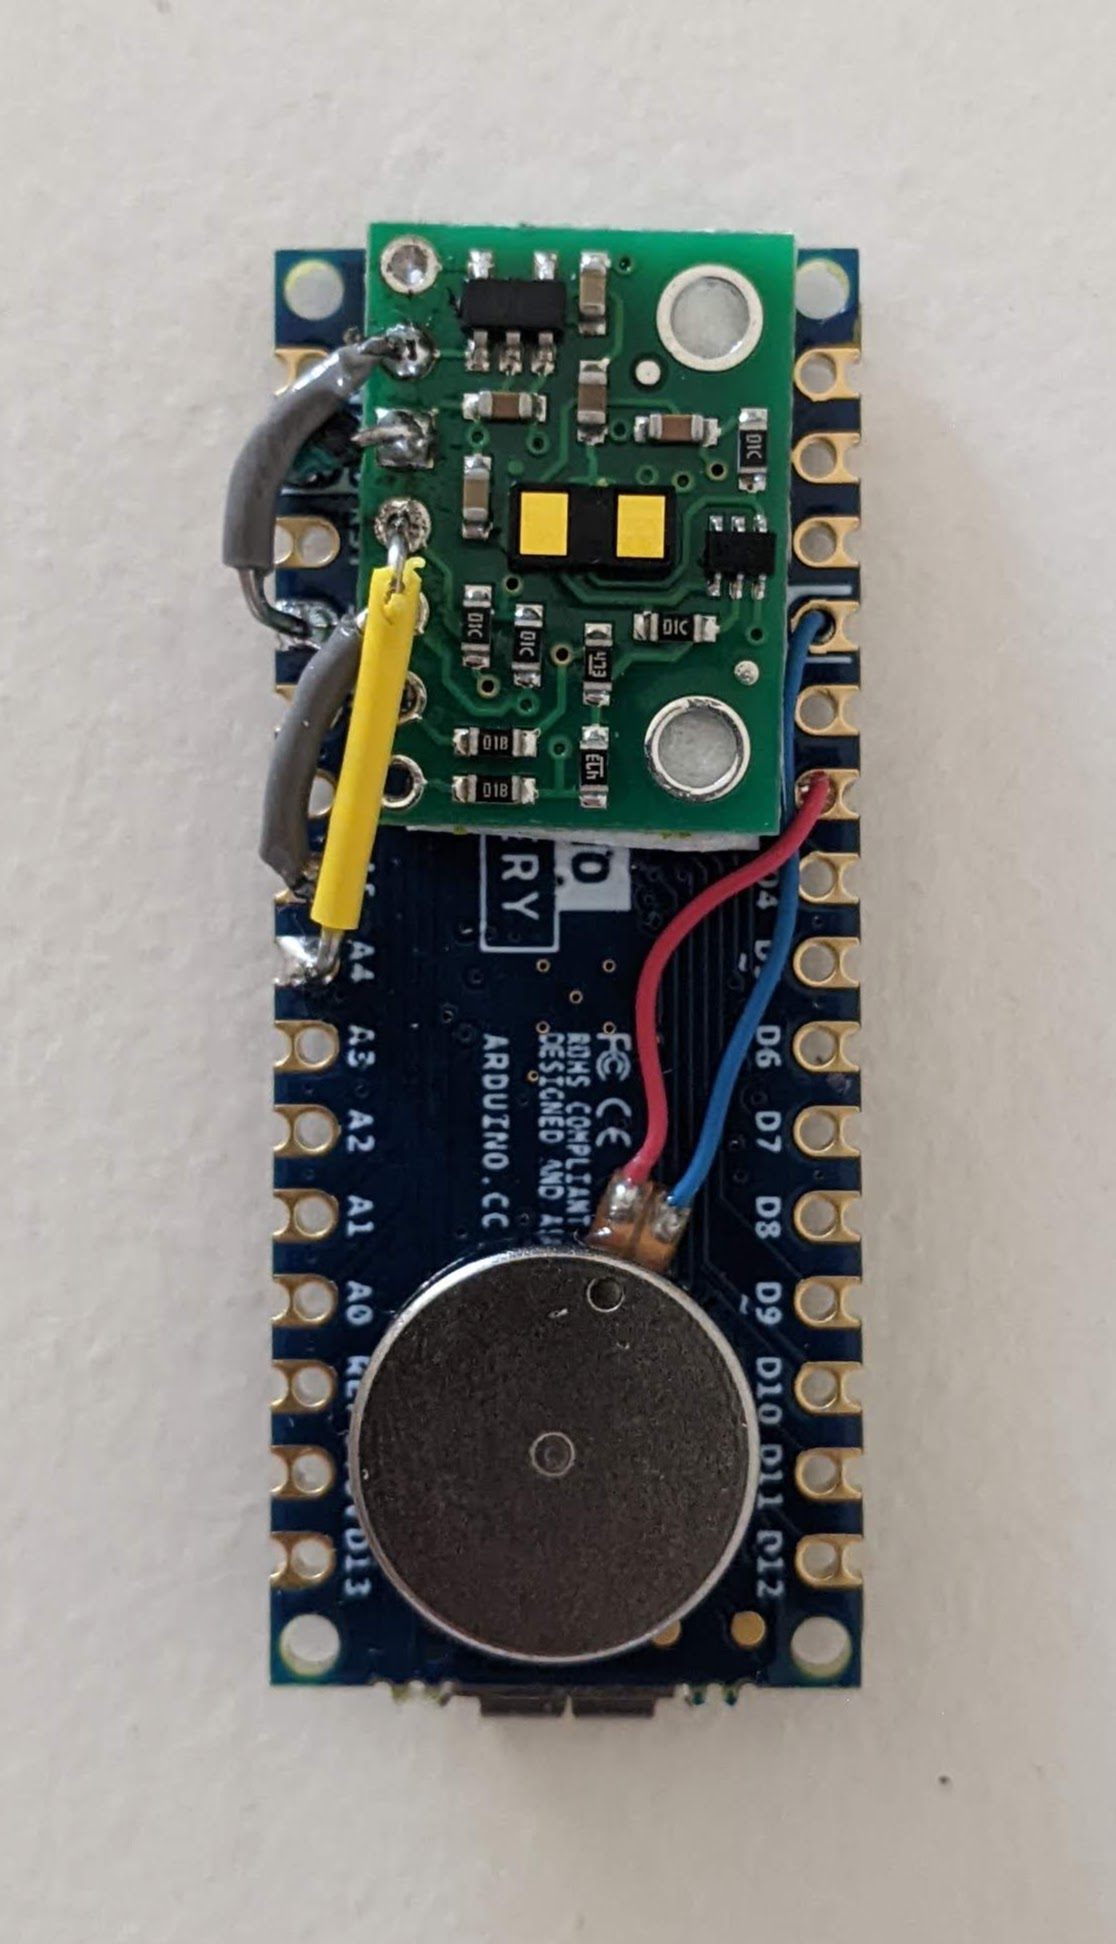
\includegraphics[height=10cm]{images/produit_fini.jpg}}}
\qquad
\subfloat[\centering Dans la main]{{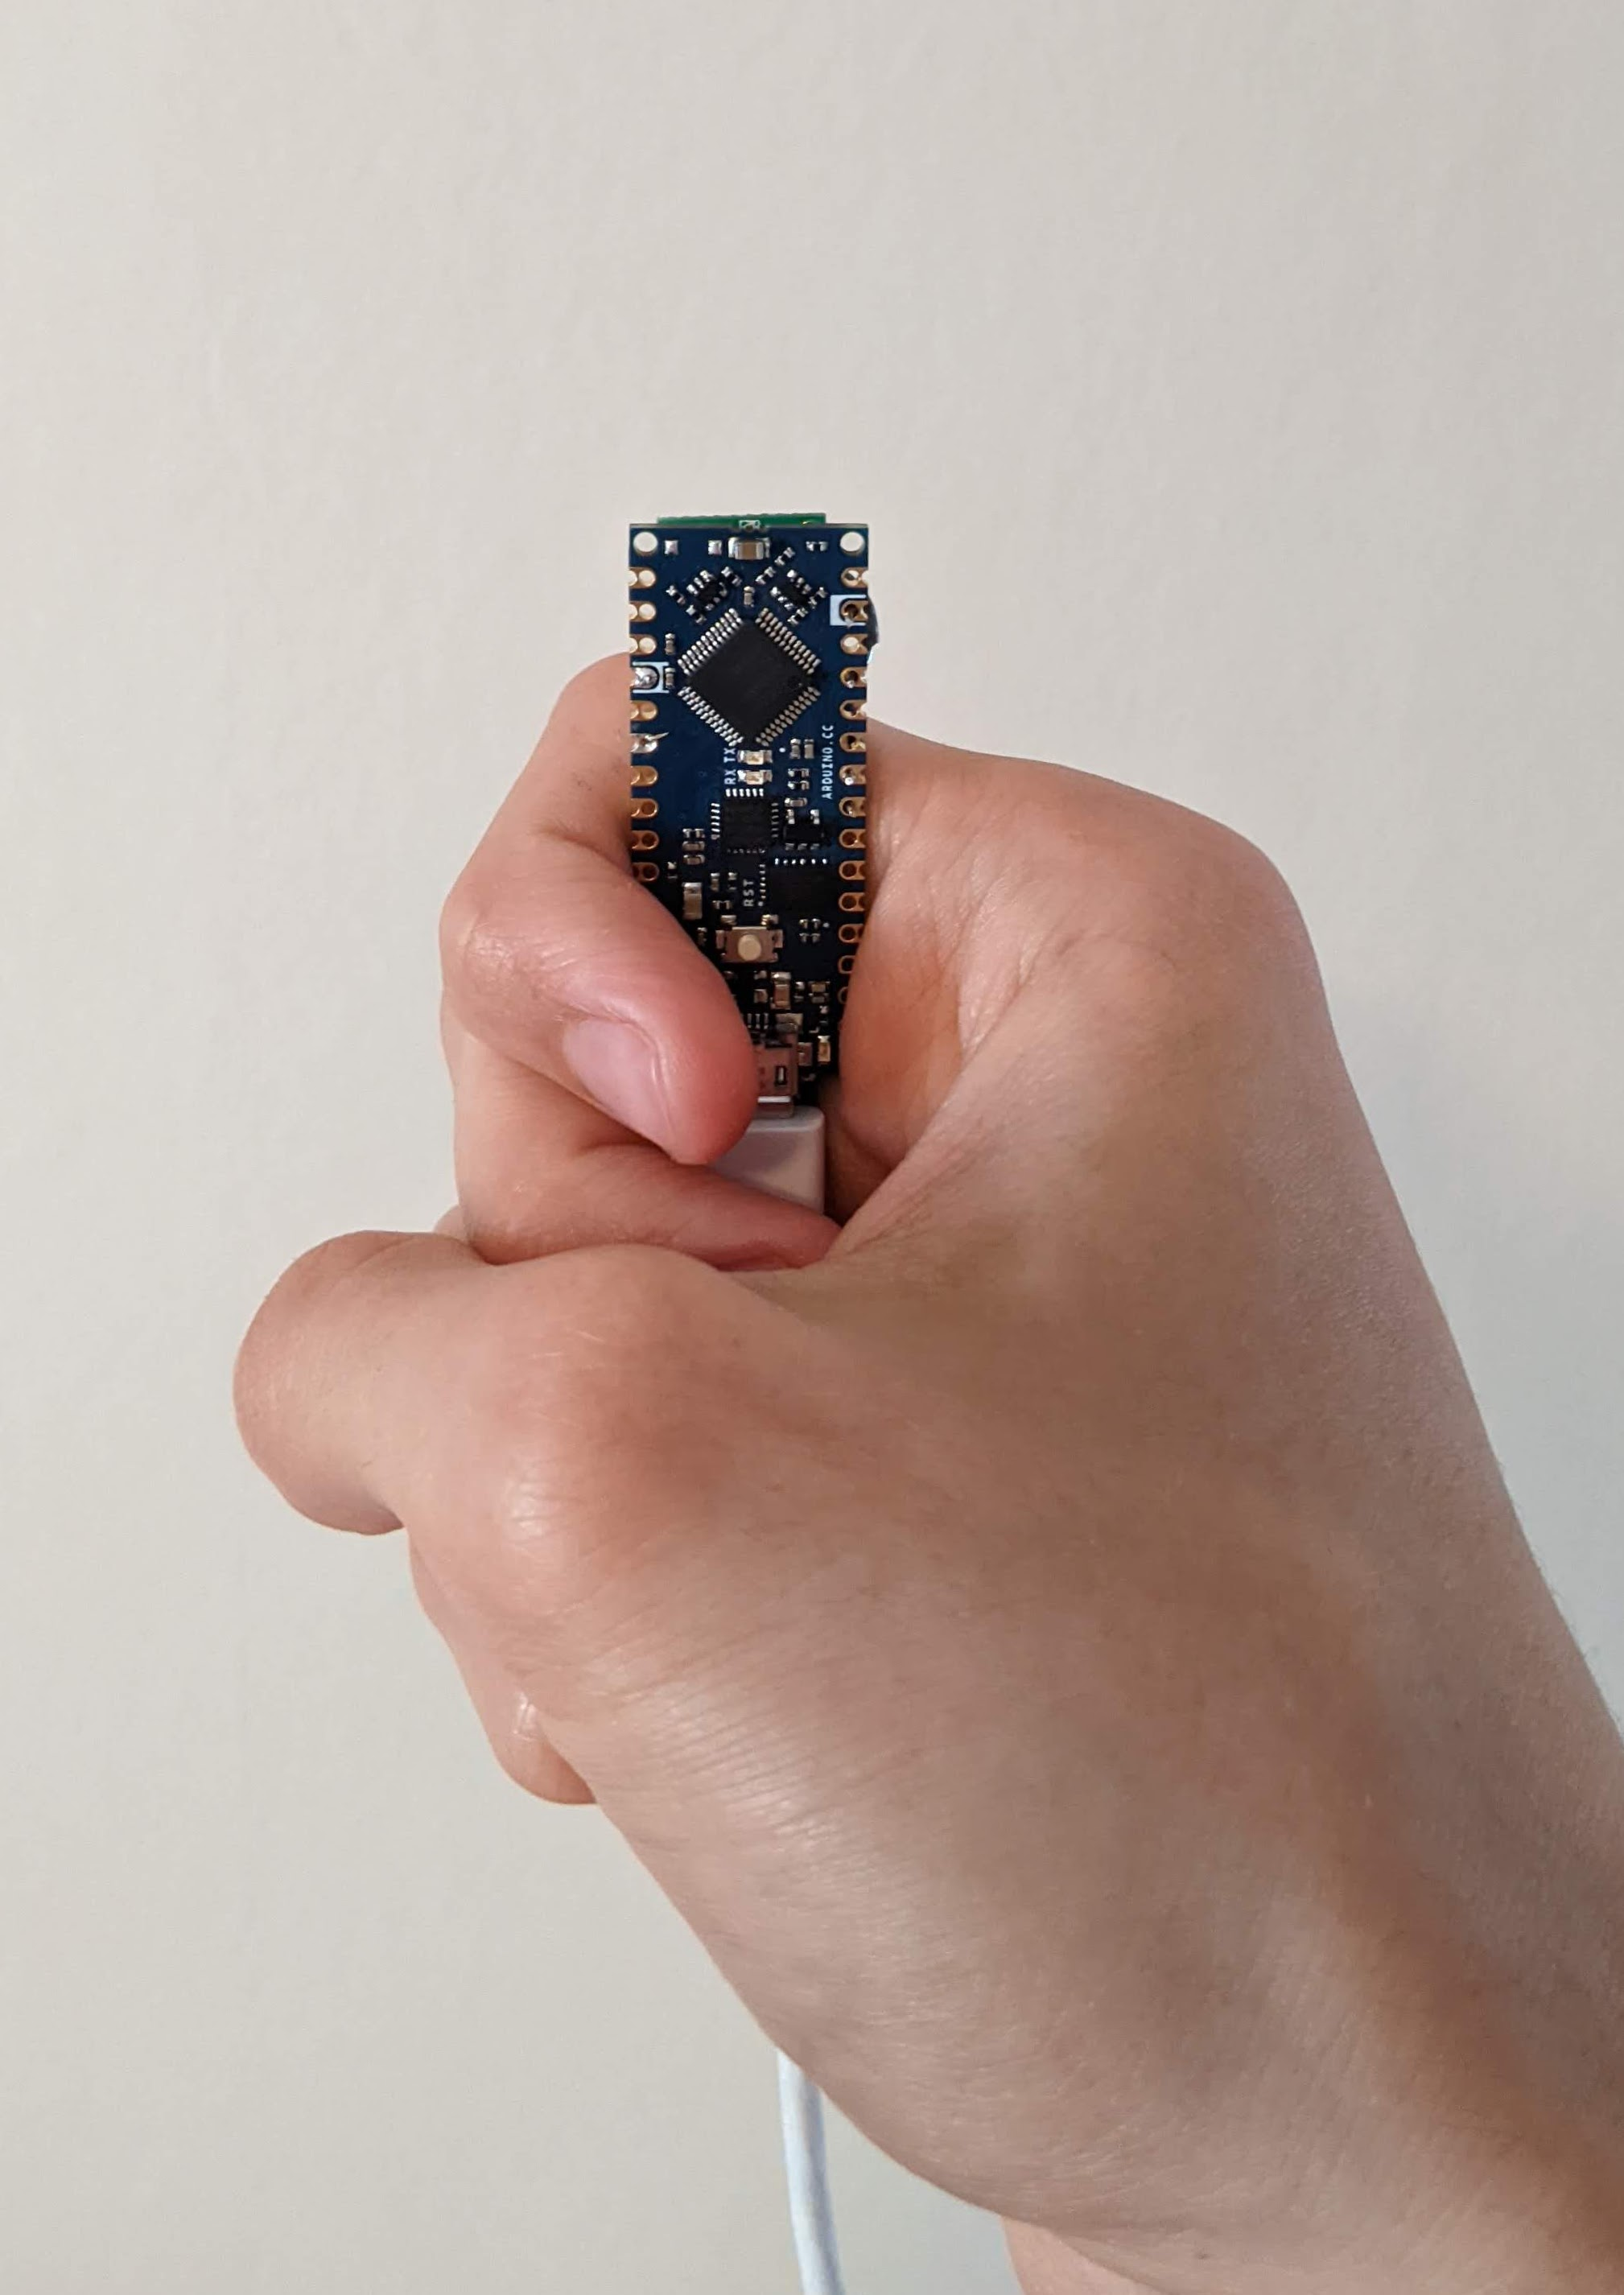
\includegraphics[height=10cm]{images/produit_fini_main.jpg}}}
\caption{Produit fini}
\end{figure}


\par Notons enfin que la rédaction et la publication de la documentation, disponible en ligne, font partie intégrante de ce projet.



%%%%%%%%%%%%%%%%%%%%%%%%%%%%%%%%%%%%%%%%%%%%%%%%%%%%%%%%%%%%%%%%%%%%%%%%%%%%%%%

\appendix

\newpage

\section{Liens}
\begin{itemize}
\item Présentation du projet : \url{https://jacquin.xyz/tipe}
\item Toutes les ressources : \url{https://github.com/arthur-jacquin/tipe}
\end{itemize}

\section{Prototype final sur {\it breadboard}}
\begin{figure}[H]
\centering
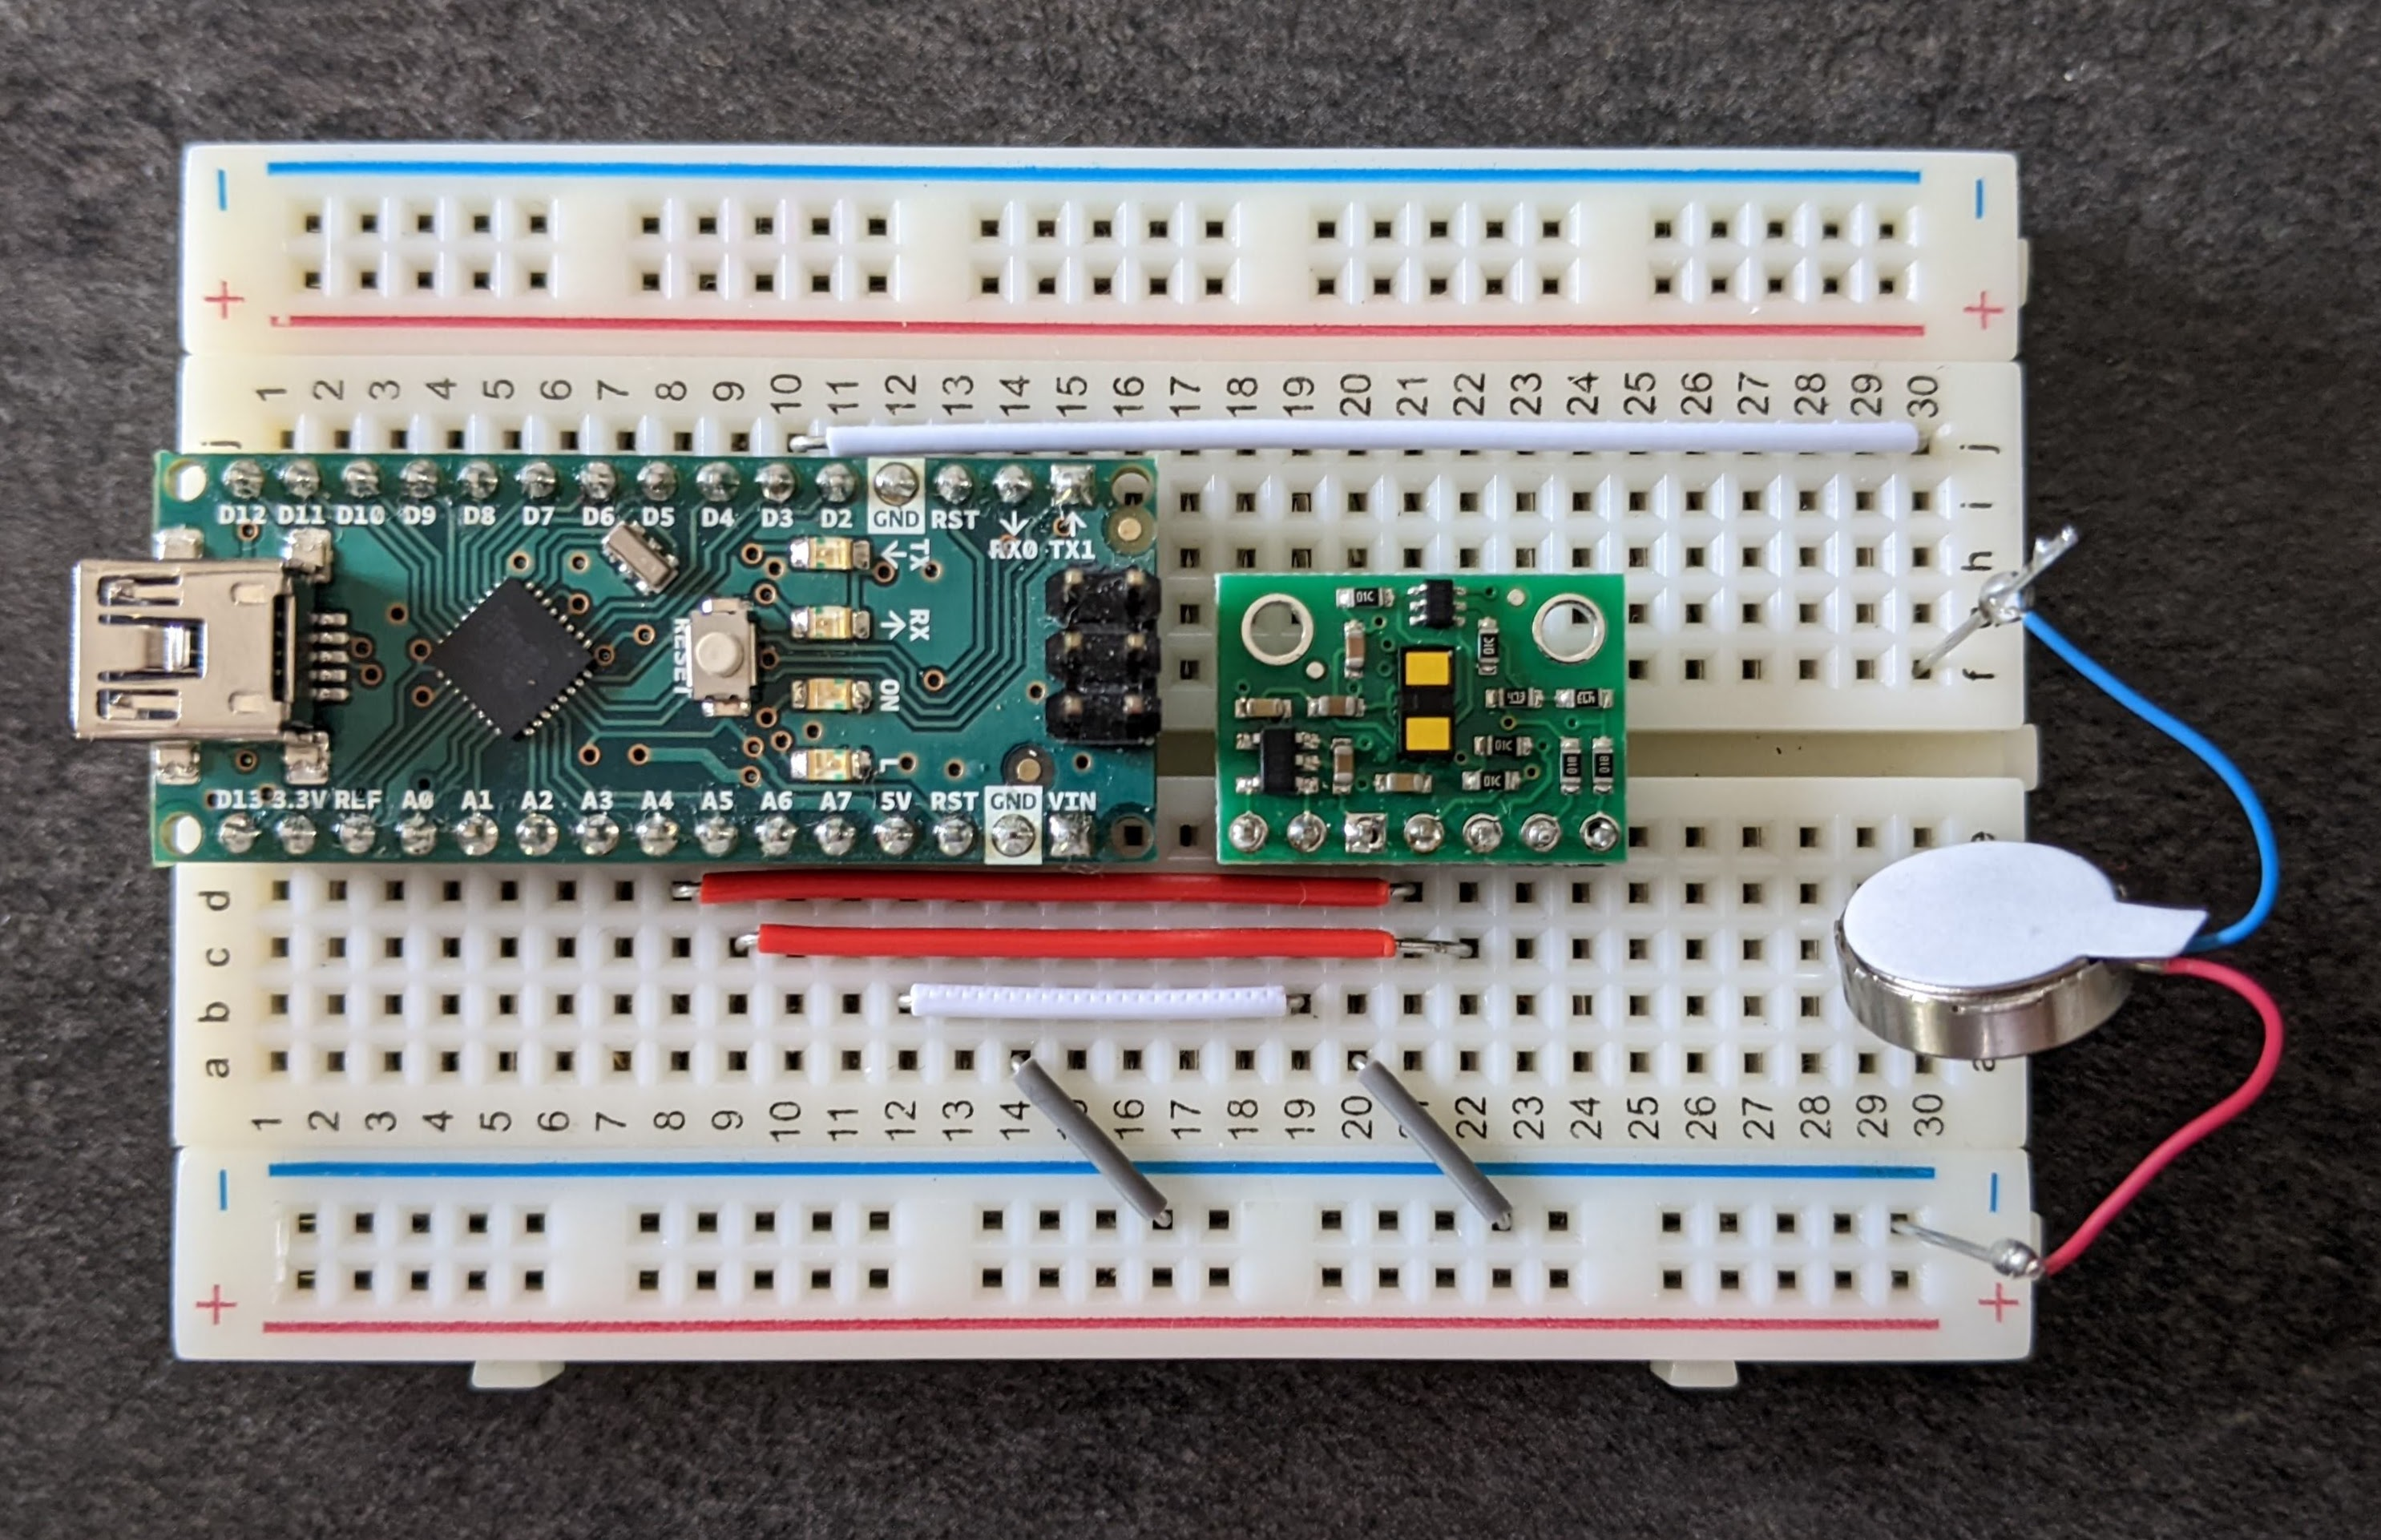
\includegraphics[width=\textwidth]{images/prototype.jpg}
\caption{Prototype final sur {\it breadboard}}
\end{figure}

\section{Code du microcontrôleur}
\lstinputlisting[language=C++]{code.ino}

\newpage

\section{Schéma électrique du VL53L1X}
\begin{figure}[H]
\centering
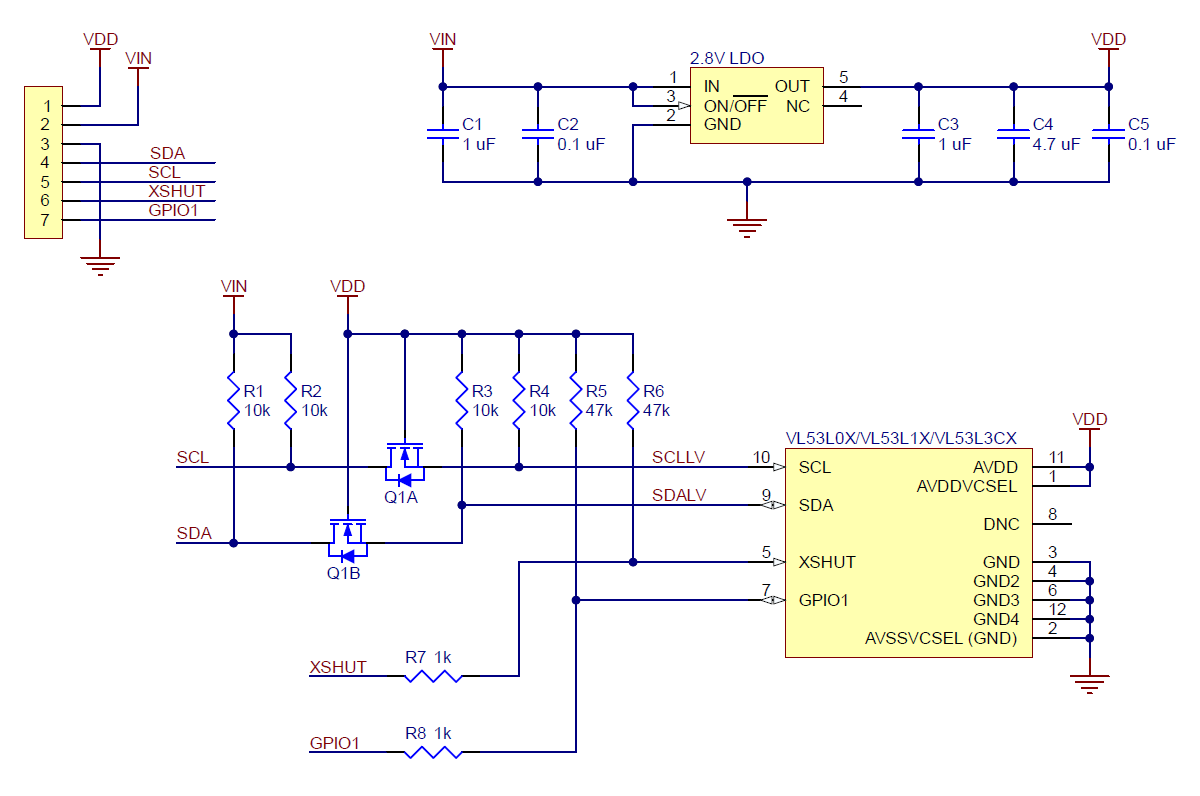
\includegraphics[width=\textwidth]{images/VL53L1X_schematic.png}
\caption{Schéma électrique du VL53L1X}
\end{figure}

\section{Liste complète des composants}
\begin{table}[h!]
\centering
\begin{scriptsize}
\begin{tabular}{ccccccr}
\hline
{\bf Catégorie} & {\bf Nom/objet} & {\bf Qté} & {\bf Fabriquant} & {\bf Réf. fabr.} & {\bf Fournisseur} & {\bf Prix (€)} \\
\hline
 & & & & & & \\
Microcontrôleur & Arduino Nano & 1 & Arduino & A000005 & Gotronic & 22,90 \\
% https://www.gotronic.fr/art-carte-arduino-nano-12422.htm
Microcontrôleur & Arduino Nano Every & 3 & Arduino & ABX00028-3P & Arduino & 25,10 \\
% https://store.arduino.cc/products/arduino-nano-every-pack
Microcontrôleur & Seeeduino XIAO & 1 & Seeedstudio & 102010328 & Gotronic & 5,90 \\
% https://www.gotronic.fr/art-seeeduino-xiao-samd21-102010328-31300.htm
Microcontrôleur & Beetle & 1 & DFRobot & DFR0282 & Gotronic & 9,80 \\
% https://www.gotronic.fr/art-carte-miniature-beetle-dfr0282-21556.htm
 & & & & & & \\
Capteur de dist. & VL53L1X & 1 & Polulu & 3415 & Gotronic & 19,40 \\
% https://www.gotronic.fr/art-capteur-de-distance-4m-3415-28058.htm
Capteur de dist. & HRLV-MaxSonar-EZ1 & 1 & Maxbotic & MB1013 & Gotronic & 39,90 \\
% https://www.gotronic.fr/art-hrlv-maxsonar-ez1-18894.htm
 & & & & & & \\
Vibreur & Vibreur miniature & 2 & Gotronic & 25355 & Gotronic & 2,60 \\
% https://www.gotronic.fr/art-vibreur-miniature-32423.htm
Vibreur & VMP2 & 1 & Solarbotics & VPM2 & Gotronic & 4,20 \\
% https://www.gotronic.fr/art-vibreur-vpm2-12006.htm
Vibreur & Gravity & 1 & DFRobot & DFR0440 & Gotronic & 2,60 \\
% https://www.gotronic.fr/art-module-vibreur-gravity-dfr0440-34310.htm
Vibreur & SMD & 1 & Seeedstudio & 316040005 & Gotronic & 1,30 \\
% https://www.gotronic.fr/art-vibreur-miniature-316040005-32651.htm
 & & & & & & \\
Prototypage & Kit plaque de montage & 1 & Gotronic & SD80A & Gotronic & 9,50 \\
% https://www.gotronic.fr/art-kit-plaque-de-montage-sd80a-25864.htm
Prototypage & Alimentation & 2 & Velleman & PS910 & Gotronic & 15,90 \\
% https://www.gotronic.fr/art-adaptateur-coude-ps910-29061.htm
Prototypage & Kit pour prototypage & 1 & Elegoo & E0 & Amazon & 20,99 \\
% https://www.amazon.fr/Elegoo-%C3%89lectronique-Breadboard-Potentiom%C3%A8tre-dapprentissage/dp/B01N0D3KTP?ref_=ast_sto_dp&th=1
 & & & & & & \\
Soudure & Station de soudage & 1 & Velleman & VTSS4N & Gotronic & 17,90 \\
% https://www.gotronic.fr/art-station-vtss4n-16972.htm
Soudure & Pompe à dessouder & 1 & Gotronic & 13580 & Gotronic & 3,50 \\
% https://www.gotronic.fr/art-pompe-a-dessouder-ppd01-7402.htm
Soudure & Fil de soudure & 1 & Gotronic & 13673 & Gotronic & 8,30 \\
% https://www.gotronic.fr/art-soudure-esp002-50-28648.htm
 & & & & & & \\
\hline
\multicolumn{6}{r}{\bf TOTAL} & 209,79 \\
\hline
\end{tabular}
\end{scriptsize}
\caption{Liste complète des composants}
\end{table}



%%%%%%%%%%%%%%%%%%%%%%%%%%%%%%%%%%%%%%%%%%%%%%%%%%%%%%%%%%%%%%%%%%%%%%%%%%%%%%%

\end{document}
